\documentclass[12pt]{article}
%Gummi|065|=)
\title{\textbf{MODULACION DE ANCHO DE PULSOS CON AMP-OPV TRANSISTORES.}}
\author{Guzman Vazquez Jaime Alan Yamil}
\date{22 de octubre}
\usepackage{graphicx}
\begin{document}
\begin{figure}[htp]
\centering

\includegraphics[scale=1.00]{/home/emile/Escritorio/guzman.vazquez.jaime.alan.yamil/tareas/EV_2_7_DISEÑO_DE_UNA_MODULACION_DE_ANCHO_DE_PULSOS_(PWM)_CON_APM_-_OPV_TRANSISTORES)/IMAGENES/índice.png}
\caption{}
\label{}
\end{figure}
\maketitle

\section{Modulacion por ancho de pulsos.}
La modulacion por ancho de pulsos conocida como PWM de fuente de energia o señal es unnatecnica en la que se modifica el ciclo de trabajo de una señal periodica para transmitir informacion a travez de un canal de comunicaciones pa o para controlar la cantidad de energia que se envia a una carga.\\
El ciclo de trabajo de una señal periodica es el ancho relativo de su parte positiva en relacion con el periodo, la formula seria la siguiente:\\\\
D=t/T\\
\\
Esto se lleva a cabo casi siempre con un circuito de PWM mediante un comparador  con dos entradas y una salida, una de las entradas se conecta a un oscilador de onda dientes de sierra, mientras que la otra queda disponible para la señal moduladora .\\
En la salida la frecuencia es generalmente igual  a la de la señal dientes de sierra y el ciclo de trabajo esta en funcion de la portadora. \\
Una de las principales desventajas que representan los circuitos PWM es la posibilidad de que haya interferencias generadas por radiofrecuencias. estas pueden minimizarse ubicando el controlador cerca de la carga realizando un filtrado de la fuente de alimentacion.\\

\begin{figure}[htp]
\centering
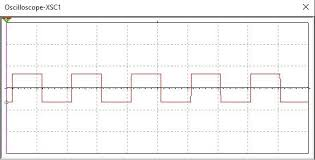
\includegraphics[scale=0.50]{/home/emile/Escritorio/guzman.vazquez.jaime.alan.yamil/tareas/EV_2_7_DISEÑO_DE_UNA_MODULACION_DE_ANCHO_DE_PULSOS_(PWM)_CON_APM_-_OPV_TRANSISTORES)/IMAGENES/onda cuadrada.jpeg}
\caption{Onda cuadrada en funcion del tiempo.}
\label{onda cuadradaa}
\end{figure}


Anteriormente observamos en la imagen (figure 2) es una onda cuadrada que son las que se genran con los PWM esta se compone de las siguientes cuestiones.\\
Las marcas en forma vertical representarian las medidas de voltaje mientras que las que estan en forma horizontal serian el tiempo, un ciclo de este tipo de onda es cuando tomas cualquier punto en el mismo y vuelves a alcanzar el mismo voltaje en la misma unidad de tiempo es decir que estos son simetricos, ejemplificando esto seria si yo tomo la parte de la esquina superior derecha de la primera onda mi marca de que el ciclo termino seria la misma esquina de la siguiente onda.\\
Este ciclo contiene practicamente dos valores uno que podriamos determinar como valor de voltaje alto y uno que seria el voltaje bajo, generalmente serian 5v para el valor alto y 0 para el valor bajo.\\
El ancho del pulso entra en este apartado, dependiendo de que tanto volataje establezcs de manera alta seria el valor ganado de voltaje o el voltaje real entregado.\\
suponiendo que en la imagen anterior (figure 2) se establecio una onda con el 50 porciento de rendimiento entonces (suponiendo que tenemos un voltaje perfecto y sin variaciones) tendriamos el 50 porciento del voltaje efectivamente es decir si el valor es de :
5 voltios entonces esto seria igual a 2.5 voltios, este seria el rednimiento real del voltaje de salida debido a que esta entregando solamente el 50 porciento del rendiiento total, este valor por supuesto puede variar dependiendo del rendimiento que le des al circuito y el volataje que se suministre.\\

 Al haber explicado el funcionamiento de la modulacion de ancho de pulso tambien podria ser preciso el nombrar las tecnicas de modulacion que existen:\\
 empezando por las tecnicas analogas se tienen tecnicas como lo serian:\\
 *AM\\
 *FM\\
 *PM\\
 *QAM\\
 *DSB\\
 *SSB\\\\
 De la modulacion digital tendriamos las siguientes tecnicas de modulacion:\\
 *ASK\\
 *APSK\\
 *FSK\\
 *CPM\\
 *GMFK\\
 *GMSK\\
 *MFSK\\
 *MSK\\
 *OOK\\
 *PPM\\
 *PSK\\
 *QAM\\
 *SC-FDMA\\
 *TCM\\\\
 Ademas de las tecnicas de modulacion anteriormente mencionadas tambien existen las tecnicas del tipo espectro disperso, cuyas configuraciones son las siguientes:\\
 *CSS\\
 *DSSS\\
 *FHSS\\
 *THSS\\
 
 
\section{Modulacion con amplificadores operacionales.}
La modulacion de el pulso por medio de los amplificadores operacionales tiene ciertas caracteristicas que se explicaran a continuacion con apoyo de la siguiente imagen.
\begin{figure}[htp]
\centering
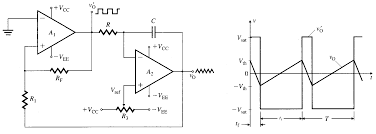
\includegraphics[scale=0.50]{/home/emile/Escritorio/guzman.vazquez.jaime.alan.yamil/tareas/EV_2_7_DISEÑO_DE_UNA_MODULACION_DE_ANCHO_DE_PULSOS_(PWM)_CON_APM_-_OPV_TRANSISTORES)/IMAGENES/señal amplificador.png}
\caption{Diagrama y grafica de señal de PWM con amplificadores operacionales.}
\label{qw}
\end{figure} 
\\

En la imagen anterior (figure 3 ) se muestra el diagrama de amplificador operacional utilizado como circuito PWM y al lado observamos la grafica corespondiente, en la salida de el segundo amplificador operacional se tiene una salida de señal triangular que se muestra en la grafica despues de que paso por el proceso del circuito y a la salida de esta misma se debe conectar una fuente de corriente directa que se muestra en la grafica, estas dos señales se van a cortar entre si por asi decirlo puesto que la señal de corriente directa esta cortando o cruzandose con la señal triangular en ciertos puntos del plano o del grafico, estos puntos se pueden interpretar como si fueran marcas para determinar en donde es que se dara el cambio de la señal ya sea de bajo a alto o vicerbersa esto forma la grafica cuadrada que se muestra dando las propiedades anteriormente mencionadas de rendimineto que se puede modular en funcion de la corriente directa que corta la señal triangular, dependiendo de donde lo corte sera el valor de amplitud de el rendimiento de la señal.\\
Esta en basicamente la forma de funcion de la modulacion de ancho de pulsos por medio de los amplificadores operacionales.\\
\\
\section{Aplicaciones}
Como lo vimos anteriormente el modular el ancho de los pulsos que enviamos puedes ser muy util para las distintas tecnologias que se pueden dar debido a que estas pueden genera por asi decirlo muchos numeros intermedios por ejemplo si tenemos un 50 porciento de eficiencia tenemos un avlor de voltaje de 2.5 suponiendo que el voltaje maximo sea 5 voltios, eso podria ser interpretado como una señal que tarnsmita una acccion o comunicacion en especifico y si tenemos una eficiencia del 10  porciento tendriamos otro valor por lo que podria ser interpretado como otra señal que dispararia otra comunicacion, esto amplificado entre todos los posibles casos de porcentajes de eficiencia, debido a esto se pueden hacer canales como la radio con cierta frecuencia dependiendo del nivel de porcentaje de eficiencia de la señal y sus modulaciones.
\section {Referencias}
knowledge.ni.com\\
ibertronica.es

\end{document}
